\documentclass{article}

% Language setting
% Replace `english' with e.g. `spanish' to change the document language
\usepackage[english]{babel}

% Set page size and margins
% Replace `letterpaper' with `a4paper' for UK/EU standard size
\usepackage[letterpaper,top=2cm,bottom=2cm,left=3cm,right=3cm,marginparwidth=1.75cm]{geometry}

% Useful packages
\usepackage{amsmath}
\usepackage{graphicx}
\usepackage[colorlinks=true, allcolors=blue]{hyperref}
\usepackage{color}
\usepackage{indentfirst}


\title{Part-of-speech Tagging}
\author{Yuanjing Zhu}

\begin{document}
\maketitle

\section{Introduction}

In PosTagging.py, I built a part-of-speech hidden markov model using the first 10,000 tagged sentences from the Brown corpus to infer the sequence of states
for sentences. First, I generated 3 matrix: initial matrix, transition matrix, and observation matrix. Then I used the provided Viterbi implementation with an OOV observation and smoothing everywhere to test the function on first 10150-10152 sentences from the Brown corpus. 

The three sentences are :

1. Those coming from other denominations will welcome the opportunity to become informed.

2. The preparatory class is an introductory face-to-face group in which new members become aquainted with one another.

3. It provides a natural transition into the life of the local church and its organizations.


\section{Result}

Comparing the result from my implementation against the truth, the accuracy is 91.5\%. There are 47 words in total, of which the model could correctly tag 43. 
\newline

\begin{tabular}{cp{12cm}c}
\centering
Sentence & POS sequence \\\hline
S1 & ['Those', 'coming', 'from', 'other', 'denominations', 'will', 'welcome', 'the', 'opportunity', 'to', 'become', 'informed', '.'] \\
S1\_Truth & ['DET', \textcolor{red}{'VERB'}, 'ADP', 'ADJ', 'NOUN', 'VERB', 'VERB', 'DET', 'NOUN', 'PRT', 'VERB', 'VERB', '.'] \\
S1\_Output & ['DET', \textcolor{red}{'NOUN'}, 'ADP', 'ADJ', 'NOUN', 'VERB', 'VERB', 'DET', 'NOUN', 'PRT', 'VERB', 'VERB', '.'] \\
S2 & ['The', 'preparatory', 'class', 'is', 'an', 'introductory', 'face-to-face', 'group', 'in', 'which', 'new', 'members', 'become', 'acquainted', 'with', 'one', 'another', '.'] \\
S2\_Truth & ['DET', 'ADJ', 'NOUN', 'VERB', 'DET', \textcolor{red}{'ADJ'}, \textcolor{red}{'ADJ'}, 'NOUN', 'ADP', 'DET', 'ADJ', 'NOUN', 'VERB', 'VERB', 'ADP', 'NUM', \textcolor{red}{'DET'}, '.'] \\
S2\_Output & ['DET', 'ADJ', 'NOUN', 'VERB', 'DET', 'NOUN', 'ADP', \textcolor{red}{'NOUN'}, \textcolor{red}{'ADP'}, 'DET', 'ADJ', 'NOUN', 'VERB', 'VERB', 'ADP', 'NUM', \textcolor{red}{'NOUN'}, '.'] \\
S3 & ['It', 'provides', 'a', 'natural', 'transition', 'into', 'the', 'life', 'of', 'the', 'local', 'church', 'and', 'its', 'organizations', '.'] \\
S3\_Truth & ['PRON', 'VERB', 'DET', 'ADJ', 'NOUN', 'ADP', 'DET', 'NOUN', 'ADP', 'DET', 'ADJ', 'NOUN', 'CONJ', 'DET', 'NOUN', '.'] \\
S3\_Output & ['PRON', 'VERB', 'DET', 'ADJ', 'NOUN', 'ADP', 'DET', 'NOUN', 'ADP', 'DET', 'ADJ', 'NOUN', 'CONJ', 'DET', 'NOUN', '.'] \\\hline
\end{tabular}
\newline
\newline
\newline
\newline
\newline
\newline
\newline


\begin{figure}[htp]
    \centering
    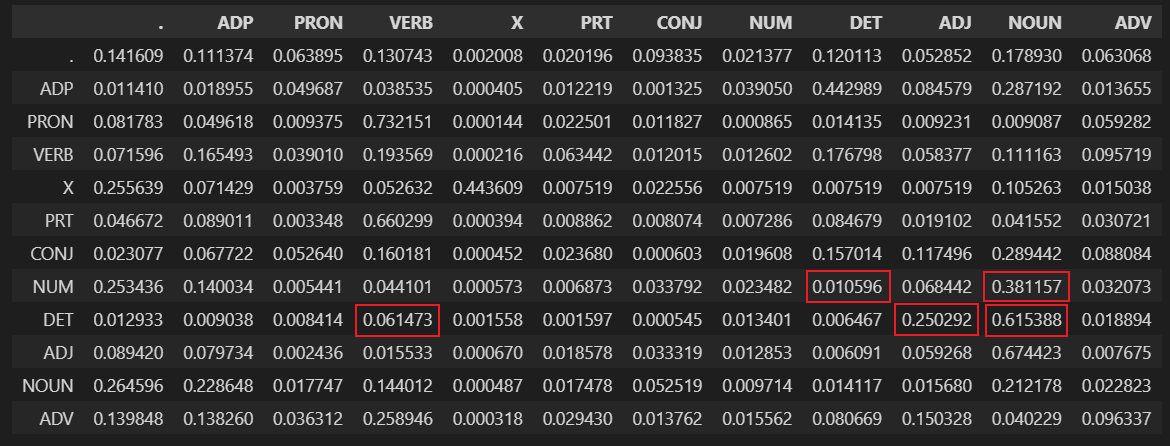
\includegraphics[width=16cm]{transition.png}
    \caption{Transition matrix}
\end{figure}

The POS tagger could generate majority of correct tags because the training samples are pretty large, total 10,000 sentences, and the 3 test sentences come from the same corpus of the training data, so the sentence structure and the frequently used words are similar. 

For the 4 mis-tagged words, the first word is "coming", it is a "VERB" but I tagged it as "NOUN". From the transition matix, we can see that the probability of a NOUN following a DET is 61.5\% while that of a VERB following a DET is only 6.14\%, so the model tends to choose NOUN to maximize the probability. For the second mis-tagged word "introductory", the reason why the model made a mistake is similar, the probability of an ADJ following a DET is 25.0\%, which is lower than the DET-NOUN combination. Next, the model failed to tag "face-to-face" as "ADJ" because it is an unknown word in the training set, so the model just identified it as "ADP" for its 22.9\% likelihood. Finally, the model mistakenly tagged "another" as NOUN which should be a DET because the probability of a DET following a NUM is pretty low, only 1.06\%.


\end{document}